\section{Evaluation} \label{sec:eval}

We compare the performance of \alg\ to the following algorithms: parallel BMW (\pBMW)~\cite{rojas2013efficient}, 
the best-in-class multiprocessor implementation we are aware of, a parallel implementation of RA (\pRA),  a shared-nothing (partitioned) parallelization of NRA (\sNRA), and a
na\"{\i}ve shared-state parallel implementation of NRA (\pNRA). 
Although our primary focus is on  approximate 
algorithms, for completeness, we also experiment with their exact counterparts.
%
% We study all these algorithms in both exact and approximate variants -- the latter over a spectrum of heuristic parameters that strike different performance-vs-recall tradeoffs.  

%In what follows, Section~\ref{ssec:setup} describes the experiment setup, Section~\ref{ssec:implementation} explains how the algorithms are implemented, and Section~\ref{ssec:results} presents our results.


\subsection{Experiment Setup}
\label{ssec:setup}

We study the algorithms in terms of query latency and throughput attainable at a single multi-core server. 
We use mid-tier industry-standard hardware -- a 12-core Intel Xeon E5620 with 24GB RAM and 1TB SSD drive. 

%\subsubsection{Evaluation Framework}

The benchmarking environment and the algorithms  are implemented in Java. 
A  \emph{benchmark driver} draws queries from an input queue and submits them to the algorithm being tested, which
% It runs the queries either one-by-one (latency mode) or in parallel (throughput mode).
%In both modes, the algorithm exploits 
uses a thread pool for intra-query parallelism. 
The driver controls the pool size. % by notifying the algorithm how many threads are available to it.
When testing latency, the thread pool is used by a single query. 
In the throughput evaluation mode, queries are scheduled first-come-first-served, 
and a new query is scheduled for execution 
once  there are idle threads with no outstanding work from currently executing queries.
All queries scheduled for execution equally share the thread pool.

In all experiments, the index is pre-built offline and stored on disk as a collection of binary files, 
each storing a shard of data partitioned by term.  The benchmark environment memory-maps the content 
of these files via a MappedByteBuffer.
Prior to each experiment, we flush the file system's page cache so all pages are physically read from disk during the experiment.
We  experiment with the TREC {\cw\/} dataset, 
Category B (ClueWeb09B) \cite{ClueWeb09}, which is widely used for information retrieval research. This dataset includes approximately 50M web documents and takes up roughly 30GB of original content, uncompressed.
We use the Lucene open-source search engine for text tokenization, posting list maintenance, 
and term statistics retrieval.
We score documents using 
a standard tf-idf score function with document length normalization~\cite{Baeza-Yates:1999:MIR:553876}. 

We draw queries from the public AOL search log.
For each number of terms from $1$ to $12$, we independently sample $100$ queries of this length uniformly at random from the AOL log.
We also  experimented with a query log of another commercial web search engine; this experiment  
produced statistically similar results, and so we omit them here.  
We use  $k=1000$. 
(Experiments with $k=100$ produced qualitatively similar results).

\subsection{Implementation}
\label{ssec:implementation}

%All algorithms store 
Posting lists are stored as contiguous uncompressed arrays;  {\pRA} also stores 
its secondary index (document id to position in the posting list mapping) in the same form. 
Term scores are stored in the posting lists as integers, scaled by $10^6$ and rounded. 
Using integer arithmetics instead of floating-point significantly speeds up document evaluation. 
The specific algorithm implementations are as follows.

\subsubsection{\pBMW}
Our implementation of {\pBMW} closely follows the description in~\cite{rojas2013distributing}. The algorithm partitions the execution of the 
sequential BMW~\cite{Ding:2011} among multiple threads. Each thread handles a distinct subset of documents, and computes a local top-k 
result. The algorithm then merges the partial results to obtain the final top-k. 
%See Section~\ref{sec:related} for detail.

Similarly to \alg, \pBMW's threads obtain jobs from a common job queue. Here, a job defines a range of document ids to scan. 
We set the number of jobs to be twice the number of worker threads, and assign equal-size ranges to all threads.  
This partition results in well-balanced execution in which the whole worker pool is utilized 
most of the time. 

Each thread maintains a thread-local heap with the current top-k documents. (We also experimented with a shared heap and 
got inferior results; a similar finding was reported in~\cite{rojas2013distributing}.)
Similarly, each thread $T$ maintains a local threshold $\Theta_T$ for filtering heap insertions; 
$\Theta_T$ is \emph{at least} the lowest score in the local heap, but may be higher thanks to the progress of other threads.  
%Specifically, threads benefit from each other's progress via a shared $\Theta$ variable. 
Thread $T$ periodically compares $\Theta$ to its local $\Theta_T$, and promotes the smaller of the two to $\max(\Theta_T, \Theta)$. 
This way,  slower workers catch up with  faster ones.

\pBMW\
%, which is applied to a segment of posting lists, further 
splits posting list segments into blocks, and uses block-level
statistics to prune the search~\cite{Ding:2011}. We experimented with multiple block sizes and selected $64$, 
which yielded the best performance.
% In 
The approximate version's pruning aggressiveness is  controlled by  a parameter 
$f \geq 1$, which multiplies $\Theta$ to obtain a higher threshold for document score upper bounds~\cite{Broder:2003}. For $f=1$, the algorithm is exact.


\subsubsection{Parallel TA variants}

\sNRA\ is a shared-nothing parallelization of NRA, where the index is partitioned to $12$ shards by document id. 
Each thread finds the top-k documents in its shard by running NRA independently with thread-local data structures. 
When all threads complete, their lists are merged and the global top-k documents are kept.  

\pNRA\ is a na\"{\i}ve shared-state parallelization of NRA that does not employ \alg's optimizations. 
Namely, it uses a shared document map, which it does not clean, and updates the term
upper bounds upon every document evaluation. As in \alg, a dedicated task checks the stopping condition.
(Distributed stopping detection yielded worse results).
{\pRA} maintains its results in a shared heap (experiments did not show any advantage to using local heaps).
Note that the algorithm's multiple worker threads may encounter postings of the same document independently, 
and consequently score that document and try to insert it into the heap multiple times. The implementation guarantees 
the uniqueness of insertion (only the first one takes effect).
Since RA's stopping detection is lightweight, we do not dedicate a task to it. Instead, all workers check the stopping condition and monitor the time elapsed since the last heap update, and notify each other if they 
decide to stop.
%A thread that detects that the algorithm can stop notifies all threads.



\subsection{Results}
\label{ssec:results}

For an algorithm A, we consider the following variants: exact (denoted A\ex), high-recall (denoted A\hi), and
low-recall (denoted A\lo). Note that the approximate algorithms' parameters ($\Delta$ and $f$) affect the recall
but do not directly control it; our high recall instances are ones that empirically achieve a  recall of $97\%$ or 
higher.


\subsubsection{Exact Algorithms}


Our first experiment shows that none of the exact algorithms meets a real-time SLA for  verbose queries. 
When processing 12-term queries with 12 worker threads (i.e., a single query fully exploits the multi-core CPU), most of the algorithms complete within 1 second. 
{\pRA} is the fastest algorithm in this setting, whereas
\pNRA\/ is much worse than the other algorithms. Its average latency exceeds 
13 seconds. For lack of space, these results are not presented here.
We will revisit the algorithms' execution dynamics -- namely, how fast they accrue their results -- 
as we study approximate algorithms in the sequel. 
 
\subsubsection{Approximate Algorithms}
 
With  exact instances of all  algorithms failing to match  real-time requirements, we turn to focus on the approximate instances. 
%Namely, 
We parameterize \alg, \pRA, \pNRA, and \sNRA\/ with $\Delta=10$ ms. 
This yields high recall in all four algorithms,  and satisfactory performance (meeting SLA requirements) in \alg. 
We instantiate \pBMW\/ with $f=5$ for high recall and $f=10$ for low recall.  

{\bf Accuracy.\ } All high-recall algorithms yield high recall (above $97\%$) and MRR-distance  (below $0.001$), while pBMW-low  suffers from low recall ($80\%$) and MRR-distance (0.048).


{\bf Latency.\ } 
Figure~\ref{fig:terms-scaling} depicts the scaling of single-query latency of the approximate algorithms  
as the number of terms scales from $1$ to $12$. The number of workers in each test 
is equal to the number of terms (for \alg, \pRA, and \pNRA, this allows maximal parallelism). 

%We also measured the $95\%$ latencies of queries on  {\cw}, which captures the so-called ``tail latency'' of the slowest $5\%$ of the queries;  \alg\/ outperformed its competitors on all query sizes. The margin was especially big for verbose queries ($5+$ terms). We omitted this result for lack of space. 


\begin{figure}[tbh]
\centering
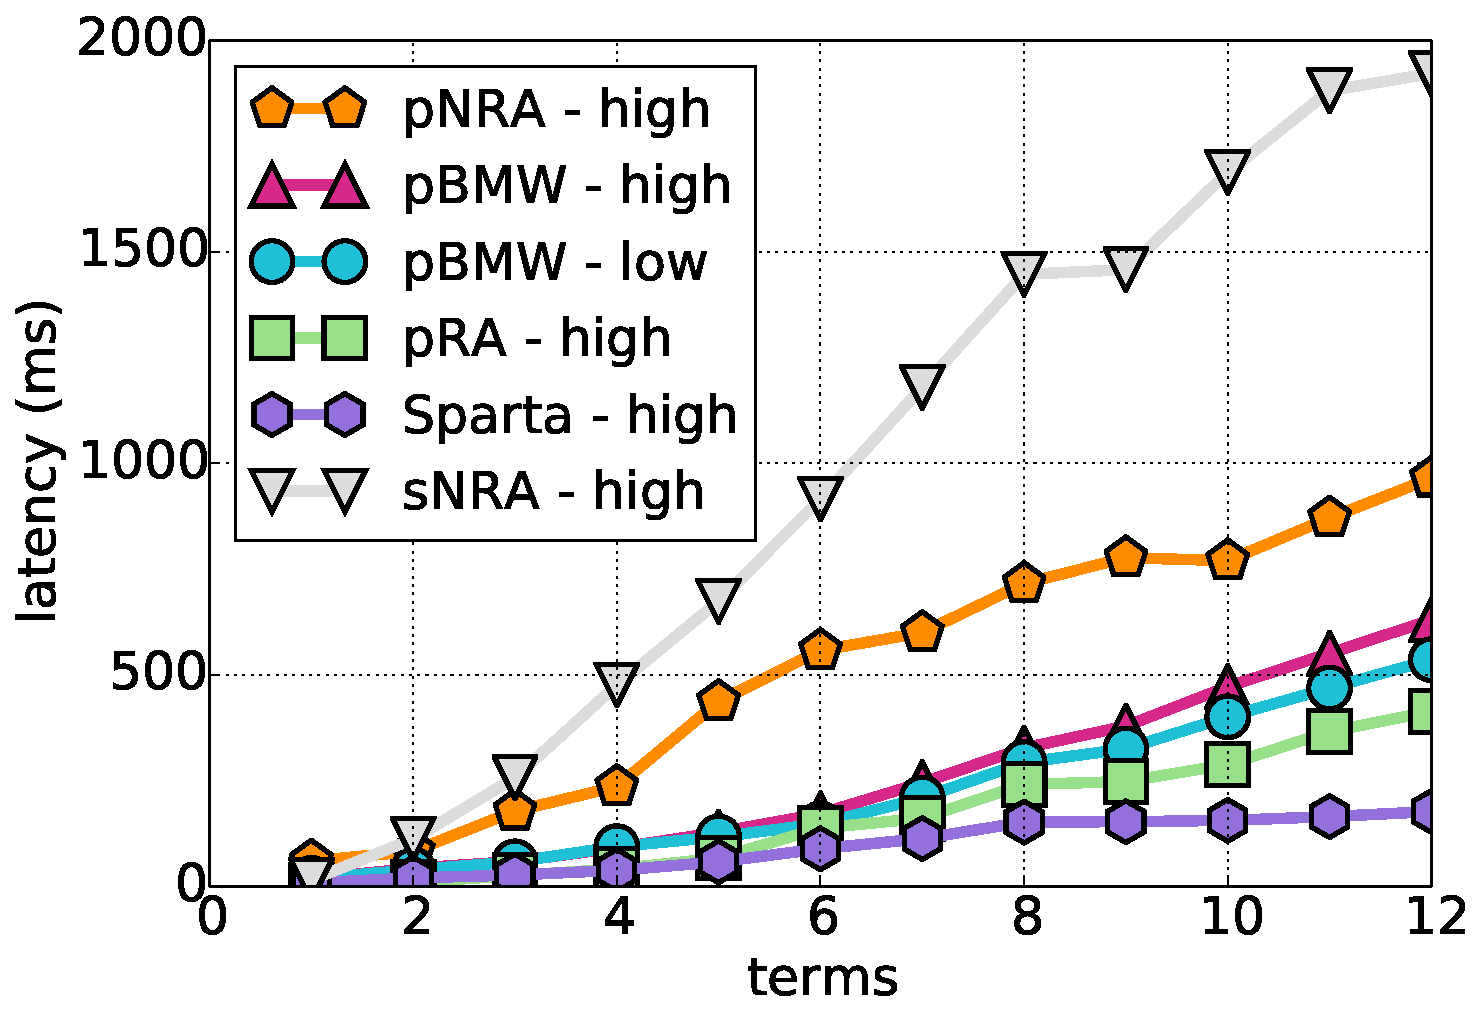
\includegraphics[width=9cm]{figures/latency_12threads_clueweb.pdf}
\caption{\small Top-k ($k=1000$) average query latency scaling with the number of query terms. 
The intra-query parallelism is equal to the number of terms. }
\label{fig:terms-scaling}
\end{figure}

\pRA\/ exhibits much weaker scalability. For example, for $12$-term queries it is slower than \alg\
by more than $2$x. We explain this by the cost of evaluating the complete 
document scores in \pRA, which forces  intensive access to the secondary index. This translates to volumes of random 
I/O that cannot be sustained even with modern SSD hardware. Note that this trend is the reverse of the one observed for \pRA\ex, 
which outperforms \alg\ex\/. That is, \alg\/ spends much more work than \pRA\/ 
in order to collect the remaining $2.5\%$ of the exact result set. We revisit this phenomenon  below. 


We see that 
\pBMW, the best-in-class algorithm in the literature, fails to match \alg's speed. For example, for 12-term queries, 
\pBMW\hi\/ completes  within $630$ ms on average. \pBMW\lo, 
which sacrifices $20\%$ of the recall for performance, only succeeds to improve these latencies by $10\%$ to $15\%$.
The shared-nothing and unoptimized parallelization of NRA are weaker than all other alternatives:
\pNRA's  average latency for 12-term queries is $1$ second, and \sNRA's is $1.7$ seconds. 
We omit \pNRA\/ and \sNRA\/ from further discussion. 

\begin{figure}[tbh]
\centering
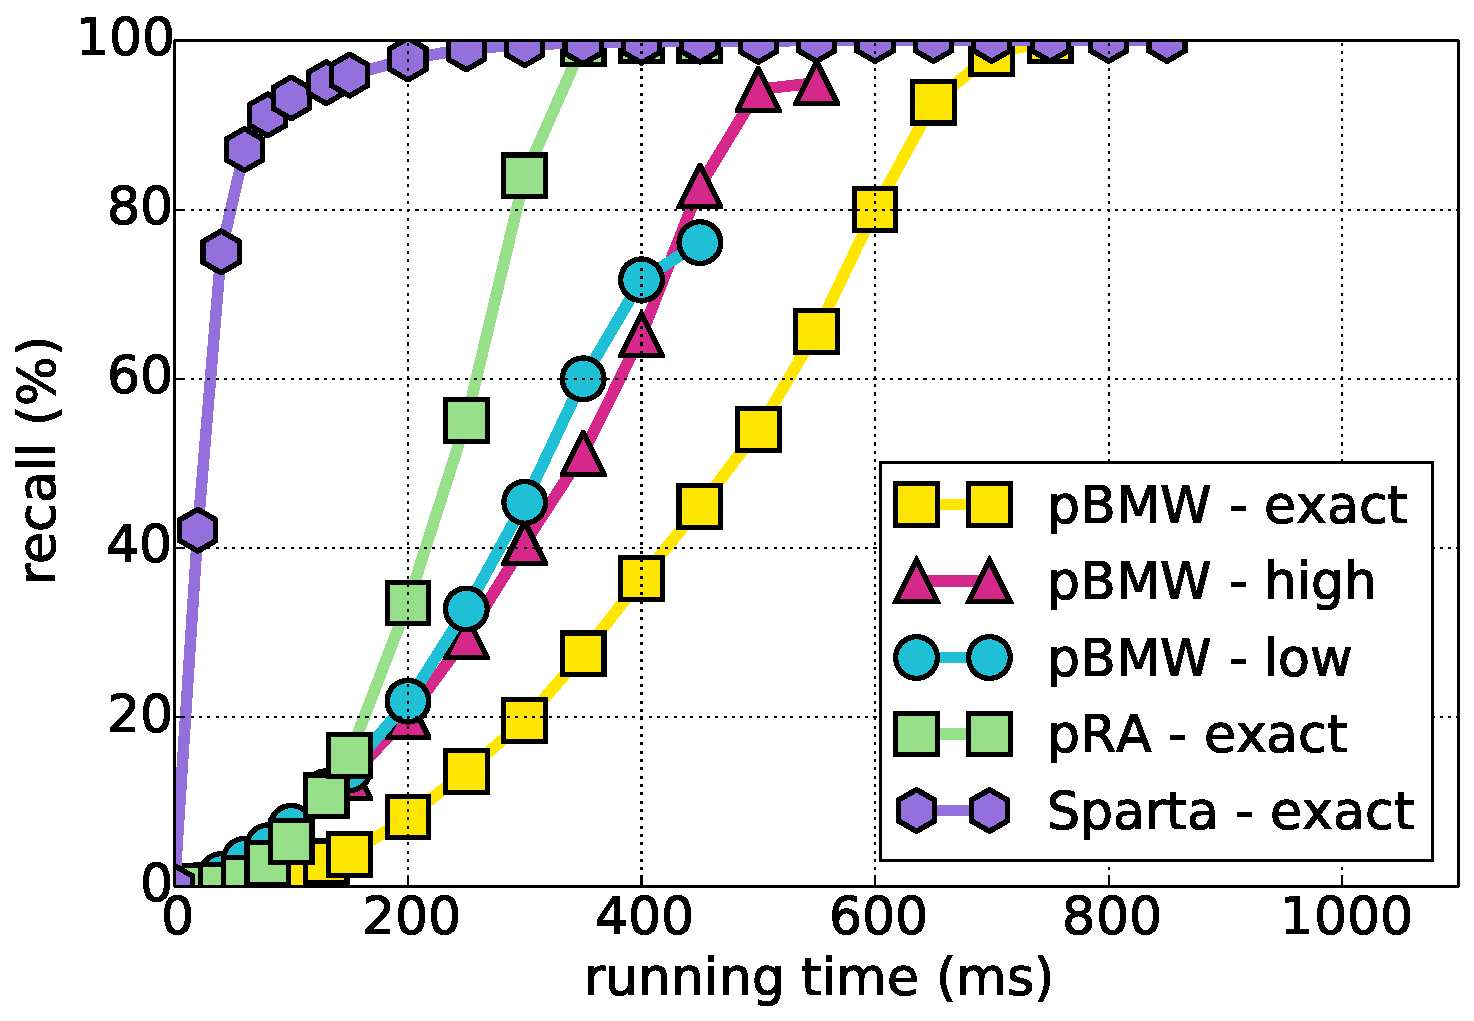
\includegraphics[width=9cm]{figures/cumulative_12threads_clueweb.pdf}
\caption{Recall dynamics with elapsed time, for 12-term queries, with 12 worker threads.}
\label{fig:dynamics}
\end{figure}

{\bf Recall dynamics.\ } 
In order to understand how the top-k results get accrued by the different algorithms, we zoom in on the dynamics of query 
recall over the running time. We focus on 12-term queries in a 12-worker configuration. 
Figure~\ref{fig:dynamics} presents the results. 
Because the approximate versions of \alg\ and \pRA\ are  identical to the respective exact versions until they stop, 
we show the dynamics of the exact versions only.  The same is not true for \pBMW, where $f$ impacts the algorithm's results from the outset.
Hence, we show the dynamics of all three instances of \pBMW. 
In the exact algorithms's curves, the rightmost data point corresponds to the exact algorithm's completion time.   

We see that \alg's recall growth is the fastest. For instance, it surpasses $80\%$ recall in less than $50$ ms, 
and $90\%$ recall in less than 100. But over time, its returns  diminish, and most of the work becomes unproductive. Whereas
\pRA\/ takes much longer to converge because it needs to fully score each encountered document,  its concluding phase is faster because 
most relevant documents   have complete  scores. 
\pBMW\/ scans the postings in the order of document ids, which is unrelated to document scores, and hence accumulates the true hits 
at a near-linear rate. Obviously, the convergence rate of \pBMW\hi\/ and \pBMW\lo\/ is faster than that of \pBMW\ex. For both datasets, the first 
two accrue results at similar rates until \pBMW\lo\/ stops at approximately $80\%$ recall. 

{\bf Parallelism.\ } 
%We next study the scaling of query latency with  intra-query parallelism. 
We next consider  $12$-term queries with a number of threads varying from $1$ to $12$. 
The results appear in Figure~\ref{fig:threads-scaling}.  The left-most data point in each curve refers to the performance of 
the respective sequential algorithm.

\alg\ requires some level of parallelism in order to achieve real-time speed, e.g., its sequential
latency is $840$ ms, which is  above typical SLA requirements. Most of the gain is achieved at low-parallelism levels (2 threads suffice). 
On the other hand, for \pBMW, much higher parallelism is essential -- its latency is inversely proportional to the number of threads. Thus, \alg\ is not only faster 
than \pBMW, but also requires less resources, which benefits throughput as we next show.

\begin{figure}[tbh]
\centering
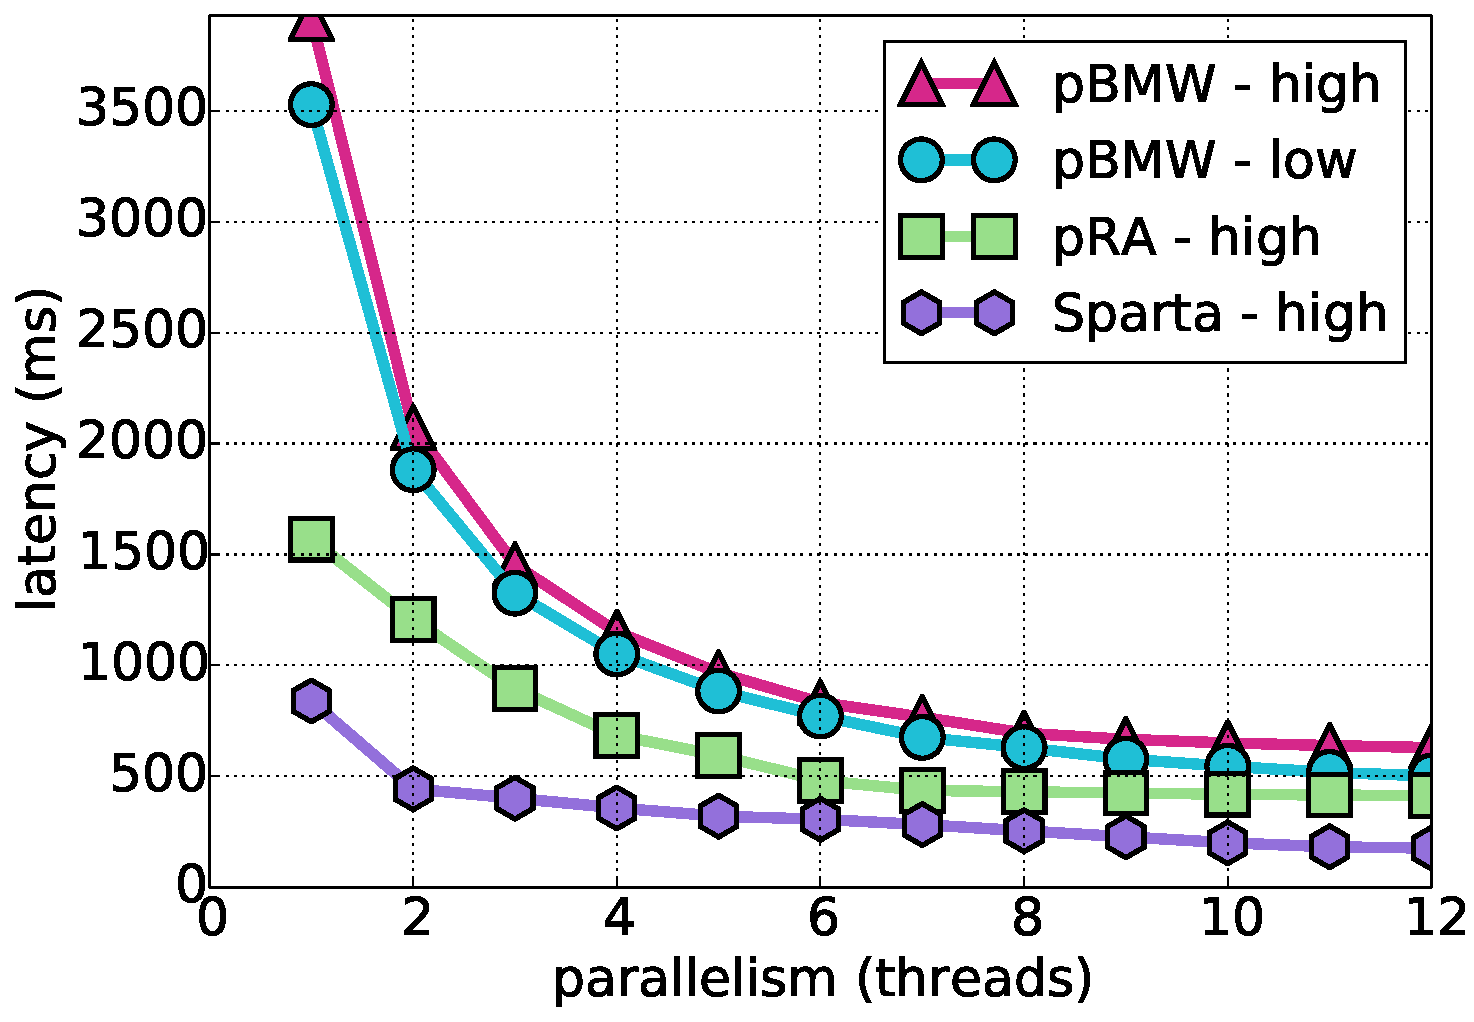
\includegraphics[width=9cm]{figures/latency_12terms_clueweb.pdf}
\caption{Top-k query latency scaling with intra-query parallelism, for $12$-term queries.}
\label{fig:threads-scaling}
\end{figure}


\begin{table}[htb]
\centering
\begin{tabular}{| c  | c | c | c | }
\hline
  \alg &  \pRA & \pBMW & \pBMW \\ 
  \hi &  \hi & \hi & \lo \\ \hline
  12.5 &  10.9 & 5.95 &  6.64 \\ 
\hline
\end{tabular}
\caption{Average throughput (in queries per second) on a query distribution measured for voice queries in production. }
\label{tab:thpt}
\end{table}

{\bf Throughput.\ } Finally, we compare the throughput (in queries per second) provided by the different
algorithms. To this end, we generate a workload with the query size distribution reported in~\cite{sigir/Guy16},
where the average query length is $4.2$ (std: $2.96$), and more than $5\%$ of the queries are $10$ terms or longer.
The queries are generated as follows: we first sample a query length $\ell$ from the distribution in~\cite{sigir/Guy16}, and then 
select a query uniformly at random among all the length-$\ell$ queries in the complete set of  $1200$ AOL queries. 

Table~\ref{tab:thpt} depicts the results of running this query mix on a shared worker pool  of $12$ threads. 
Here too, \alg\/ improves over its competitors by a wide margin. This  advantage is thanks to a combination of \alg's speed and lower resource utilization.

 